\section{Kvalitetssikring}

\begin{frame}
	\frametitle{Usabilityfejl}
  \begin{itemize}
    \item Tænk-højt sessions vha.\ cases
    \item Resultat
    \begin{itemize}
      \item Forbedret funktionalitet
      \item Forbedret brugergrænsefladedesign
    \end{itemize}
  \end{itemize}
\end{frame}

\begin{frame}
	\frametitle{Instant Data Analysis}
  \begin{itemize}
    \item Hvad er det?
	  \item Setup
      % 3 gruppemedlemmer i feltet, 3 i grupperummet
      % Fik informant til at gennemgå case
      % 6 mannetimer pr. informant
    \item Fejltyper
      \begin{itemize}
        \item Kritiske
        \item Seriøse
        \item Kosmetiske
      \end{itemize}
  \end{itemize}
\end{frame}

\begin{frame}[fragile]
  \begin{figure}
  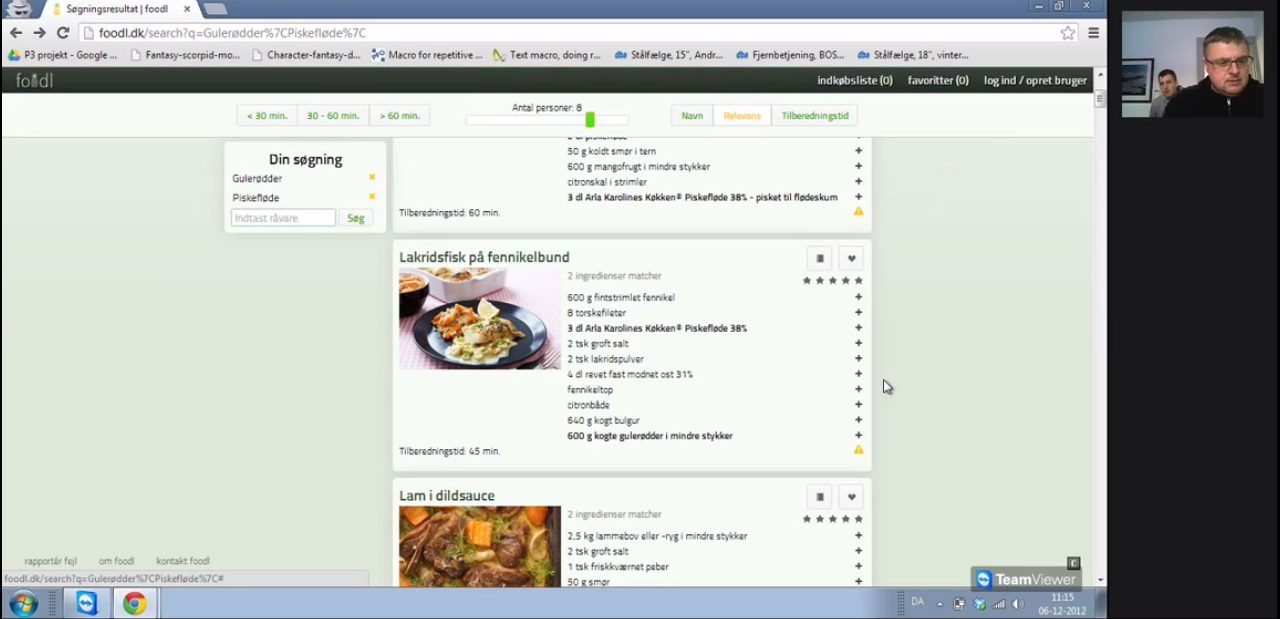
\includegraphics[width=\textwidth]{billeder/keldIDA.png}
  \end{figure}
\end{frame}

\begin{frame}
	\frametitle{Fundne usabilityfejl}
    \begin{itemize}
	  \item Indkøbsliste (1 kritisk, 5 kosmetiske)
    \item Søgning (2 seriøse, 1 kritisk)
    \item Søgeresultat (1 seriøs)
    \item Sidehoved og toolbar (5 seriøse)
    \item Favorisering (1 kosmetisk)
    \item Kontakt os (1 seriøs)
  \end{itemize}
\end{frame}

\begin{frame}
  \frametitle{Unit test}
  \begin{itemize}
    \item Webapplikation
    \item Dataudtrækker
    \item Var det nok?
  \end{itemize}
\end{frame}
